\section{Shuffle Optimization}
\label{opt}
This section presents the detailed methodologies to achieve the three design goals. 
The out-of-framework shuffle data management is used to decouple shuffle from execution and provide a cross-framework optimization. 
Two heuristic algorithms (Algorithm \ref{hminheap}, \ref{mhminheap}) and a co-scheduler is used to achieve shuffle data pre-fetching without launching tasks.

\begin{figure}
    \centering
    % \begin{minipage}{0.42\textwidth}
    %     \centering
    %     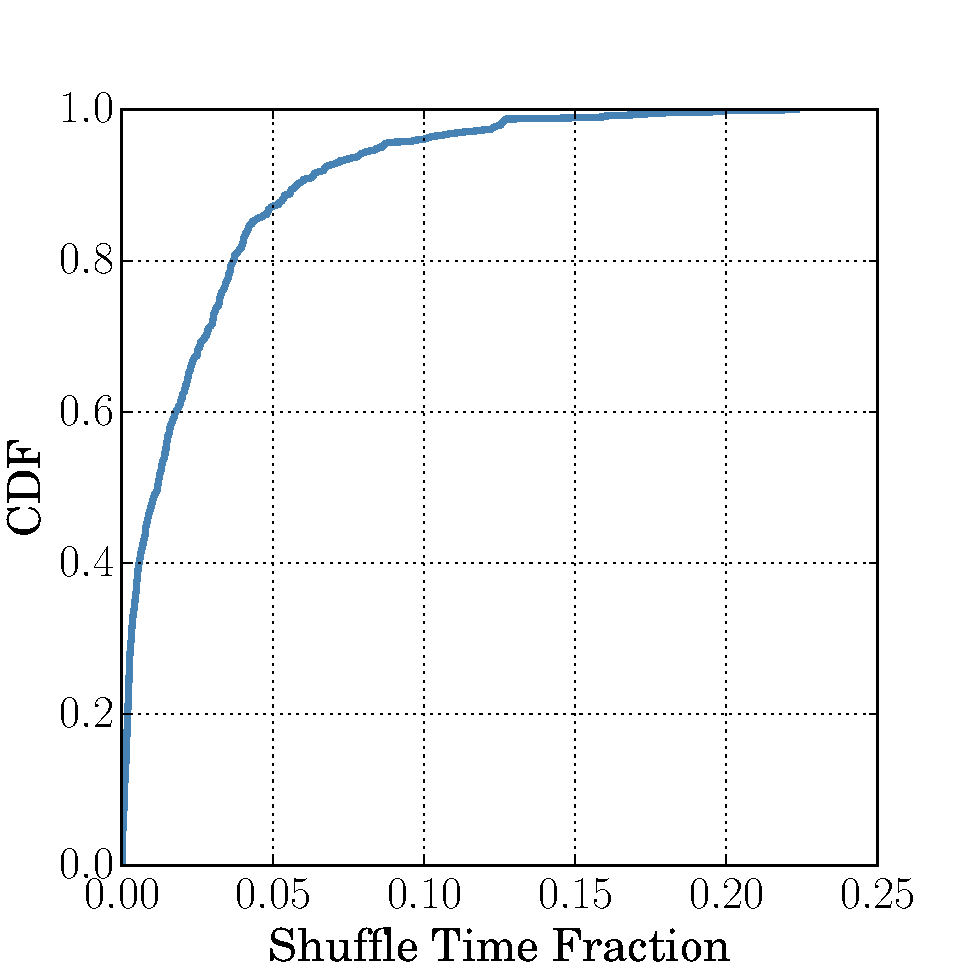
\includegraphics[width=0.9\textwidth]{fig/reduce_cdf} % first figure itself
	% 	\caption{Shuffle Time Fraction CDF of OpenCloud Trace}
	% 	\label{fig:cdf}
    % \end{minipage}\hfill
    \begin{minipage}{0.42\textwidth}
        \centering
        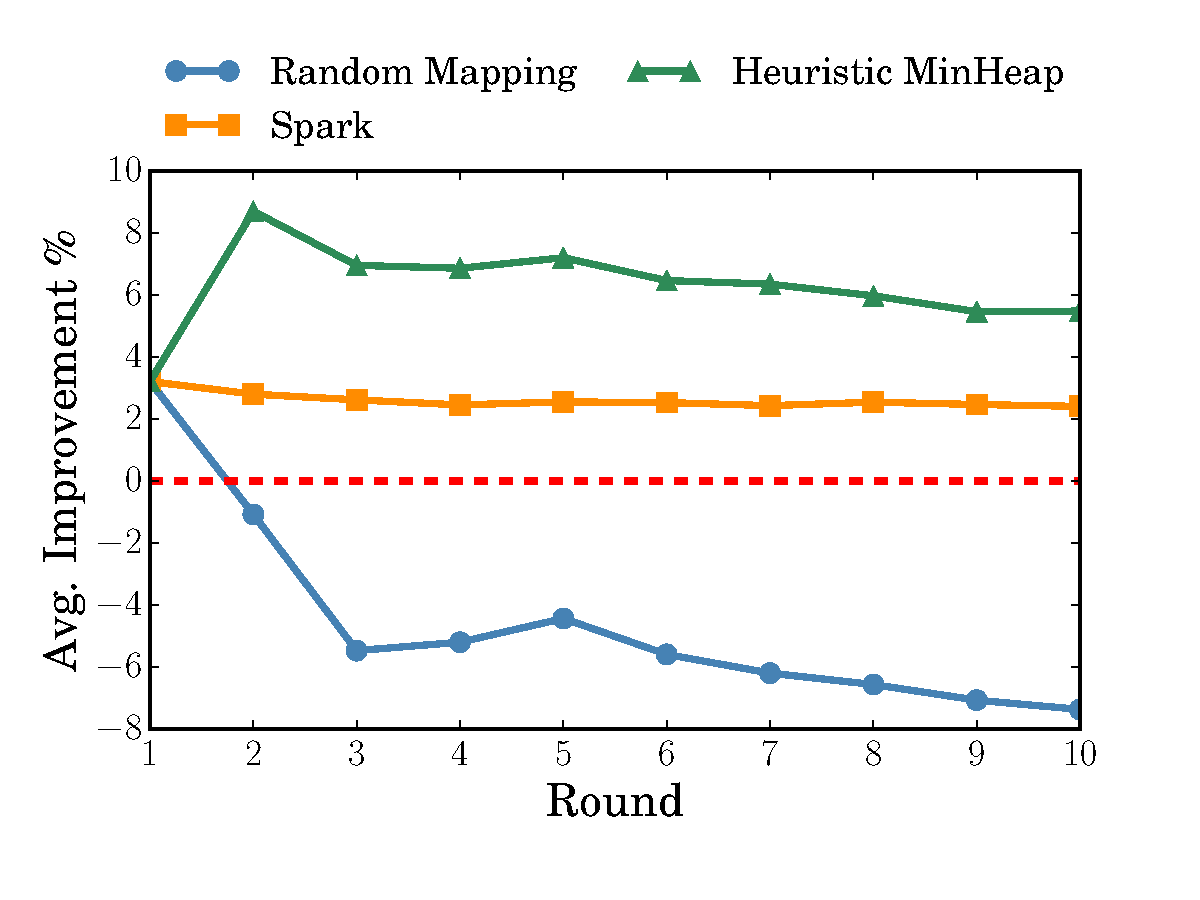
\includegraphics[width=\textwidth]{fig/sim} % second figure itself
		\caption{Stage Completion Time Improvement of OpenCloud Trace}
		\label{fig:sim}
	\end{minipage}
	\begin{minipage}{0.49\textwidth}
        \centering
        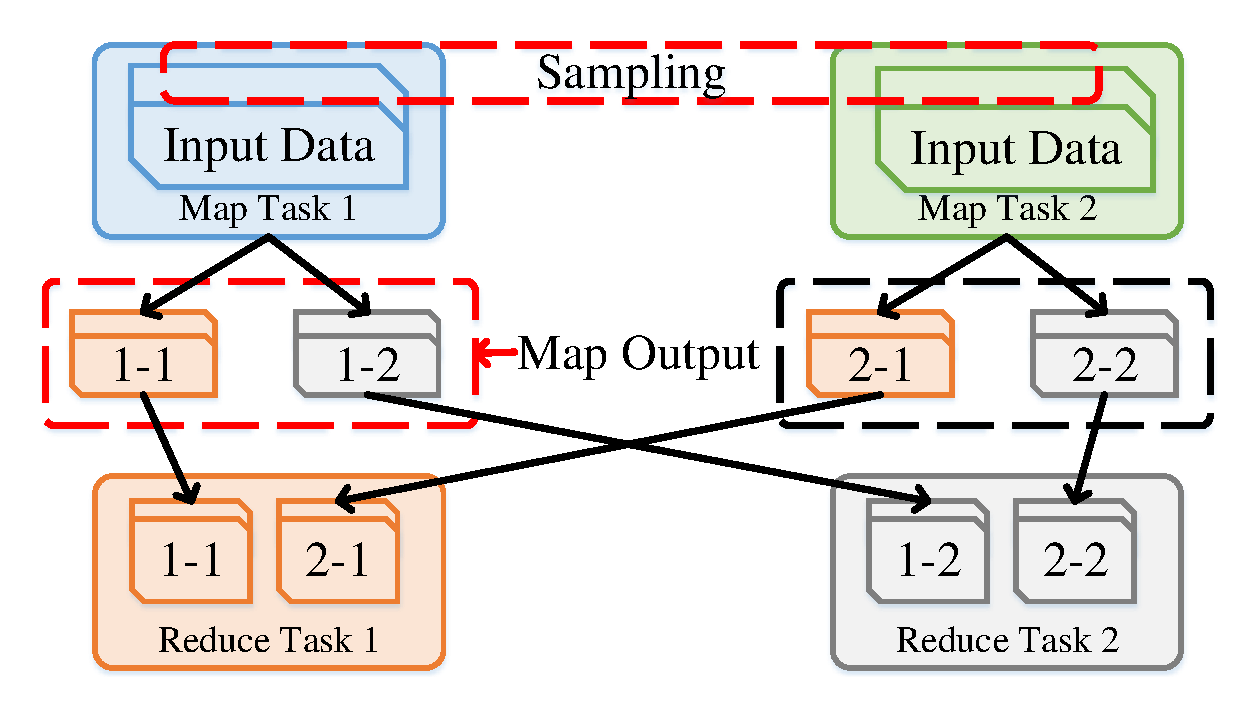
\includegraphics[width=0.9\textwidth]{fig/shuffle} % first figure itself
		\caption{Shuffle Data Prediction}
		\label{fig:shuffle}
    \end{minipage}\hfill
\end{figure}

\subsection{Decouple Shuffle from Execution}
% \ifrevision
% \reversemarginpar
% \marginpar{B1,C2}
% \fi
To achieve the decoupling of map tasks and reduce tasks, the original shuffle write and read implementation in the current frameworks should be modified to apply the API of SCache.
% During shuffle write of map tasks, the partitioned shuffle data blocks will be written on the disks.
% Each block contains a part of input data of a particular reduce task. 
To prevent the release of a slot being blocked by shuffle write,  
SCache provides a disk-write-like API named $putBlock$ to handle the storage of partitioned shuffle data blocks produced by a map task.
Inside the $putBlock$, SCache uses memory copy to move the shuffle data blocks out of map tasks and store them in the reserved memory.
After the memory copy, the slot will be released immediately.

From the perspective of reduce task, SCache provides an API named $getBlock$ to replace the original implementation of shuffle read. 
With the precondition of shuffle data pre-fetching, 
the $getBlock$ leverages the memory copy to fetch the shuffle data from the local memory of SCache.
% Instead, the original implementation of shuffle read will trigger an all-to-all network transfer that keeps CPU idle.
%To this end, all I/O operations are managed outside of the DAG framework, and the slot is occupied only by the CPU intensive phases of task.
\subsection{Pre-schedule with Application Context}
The pre-scheduling and pre-fetching are the most critical aspects of the optimization. 
The task-node mapping is not determined until tasks are scheduled by the scheduler of DAG framework. 
Once the tasks are scheduled, the slots will be occupied to launch them. 
On the other hand, the shuffle data cannot be pre-fetched without the awareness of task-node mapping.
We propose a co-scheduling scheme with two heuristic algorithms (Algorithm \ref{hminheap}, \ref{mhminheap}). 
That is, the task-node mapping is established a priori, and then it is enforced by the co-scheduler when the DAG framework starts task scheduling. 
% We explore several pre-scheduling schemes in different scenarios, and evaluate the performance calculating the improvement of reduce tasks completion time with trace of OpenCloud \cite{opencloudtrace}. We first emulate the scheduling algorithm of Spark to schedule the reduce tasks of one job, and take the bottleneck of the task set as the completion time. Then we remove the shuffle read time as the assumption of shuffle data pre-fetch and emulate under different schemes. The result is shown in \ref{fig:sim}.
% \begin{figure*}
% 	\centering
% 	\begin{minipage}{0.34\linewidth}
% 		\begin{figure}[H]
% 			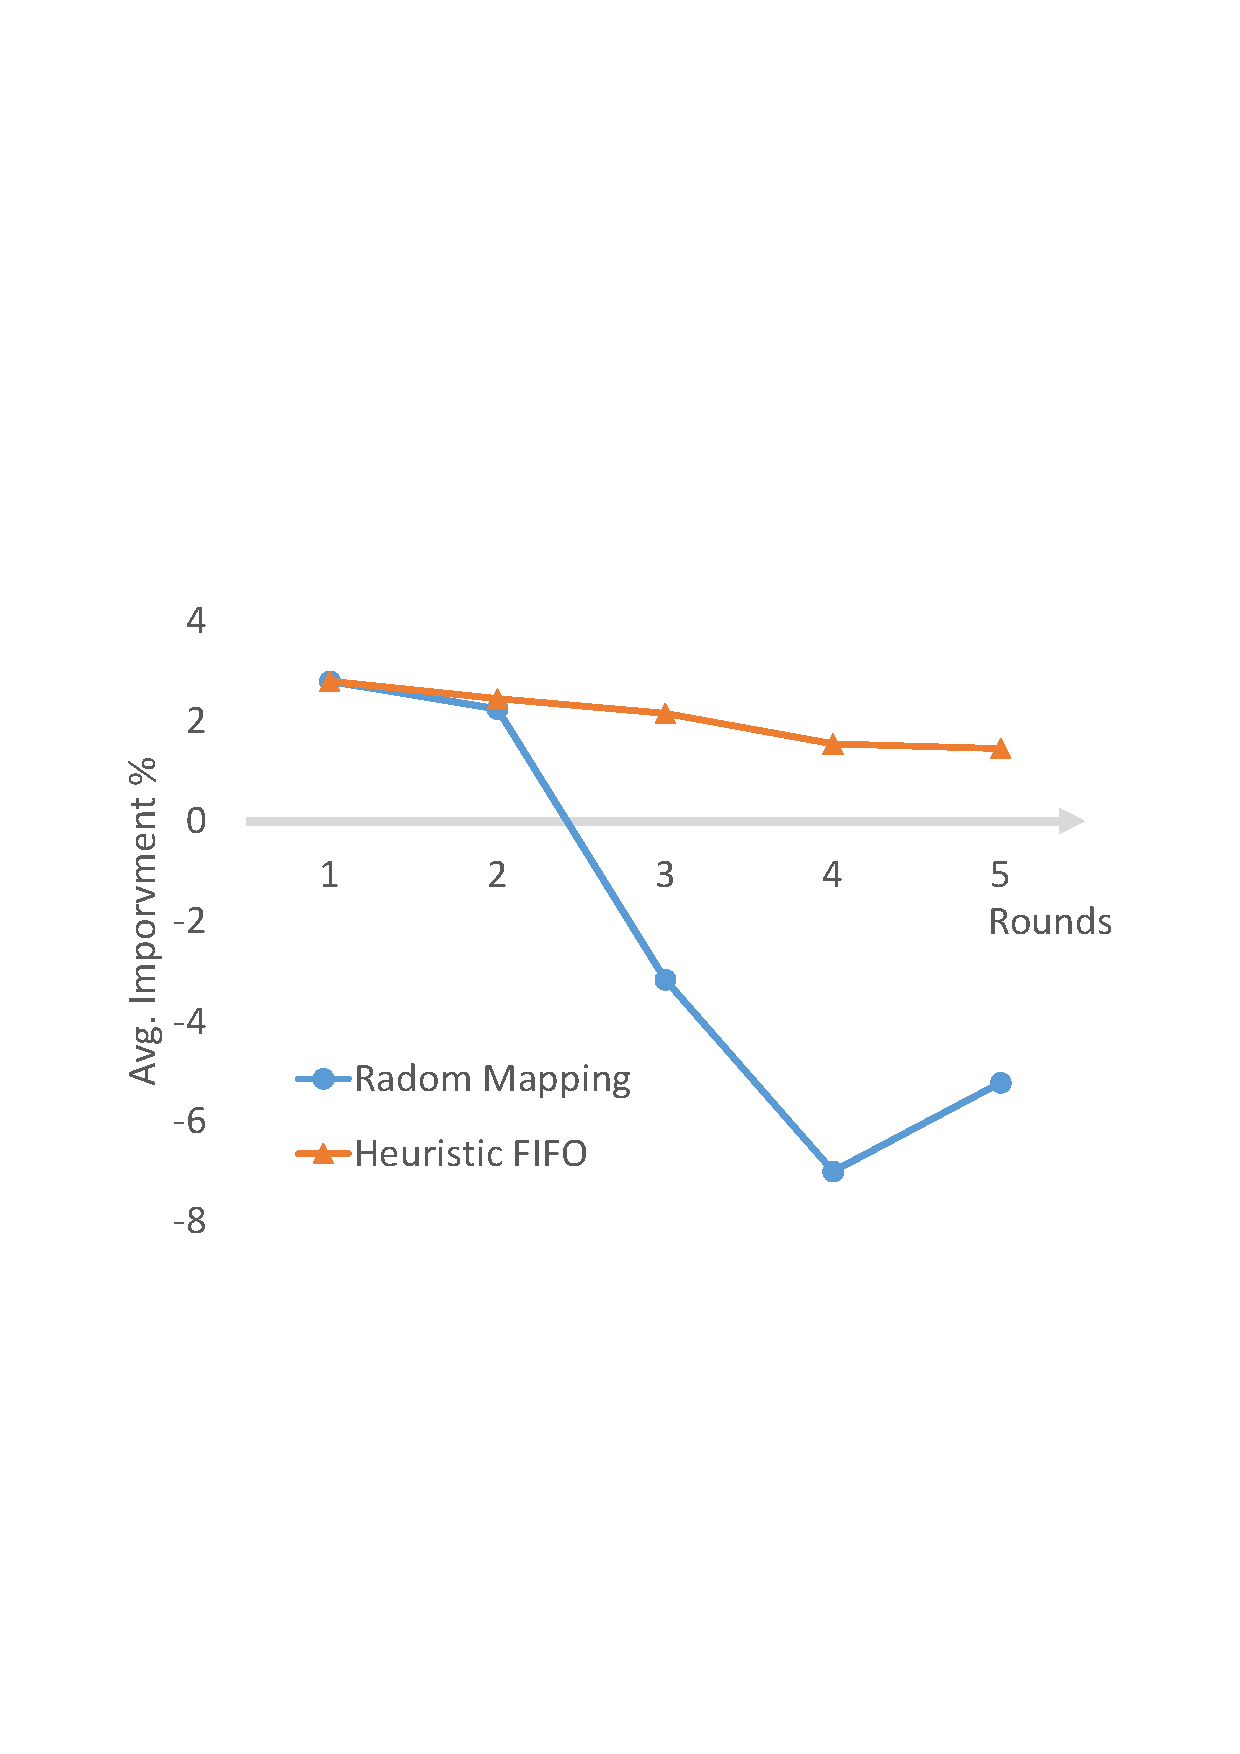
\includegraphics[width=\textwidth]{fig/shuffle_size}
% 			\caption{Shuffle Size Comparing with Input Size}
% 			\label{fig:shuffle_size}
% 		\end{figure}
% 	\end{minipage}
% 	\begin{minipage}{0.65\linewidth}
% 		\begin{figure}[H]
% 			\begin{subfigure}{0.5\textwidth}
% 				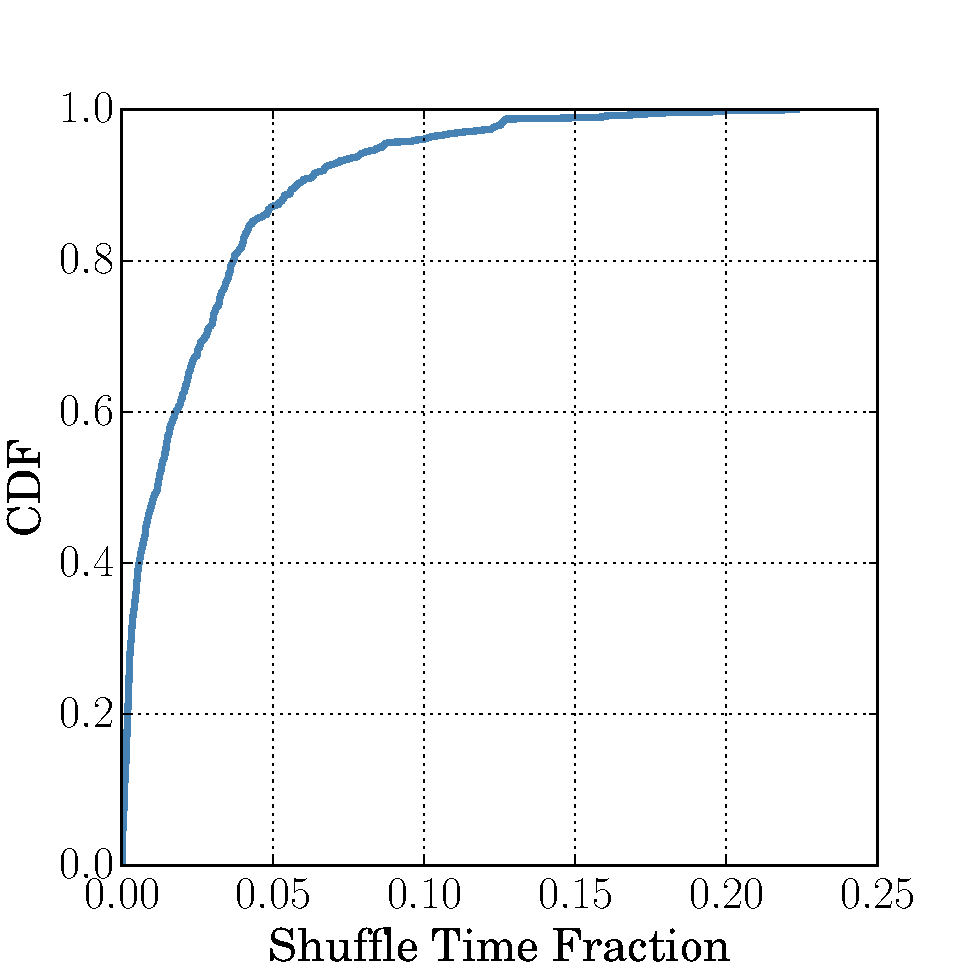
\includegraphics[width=\linewidth]{fig/reduce_cdf}
% 				\caption{Shuffle Time Fraction CDF}
% 				\label{fig:cdf}
% 			\end{subfigure}	
% 			\begin{subfigure}{0.5\textwidth}
% 				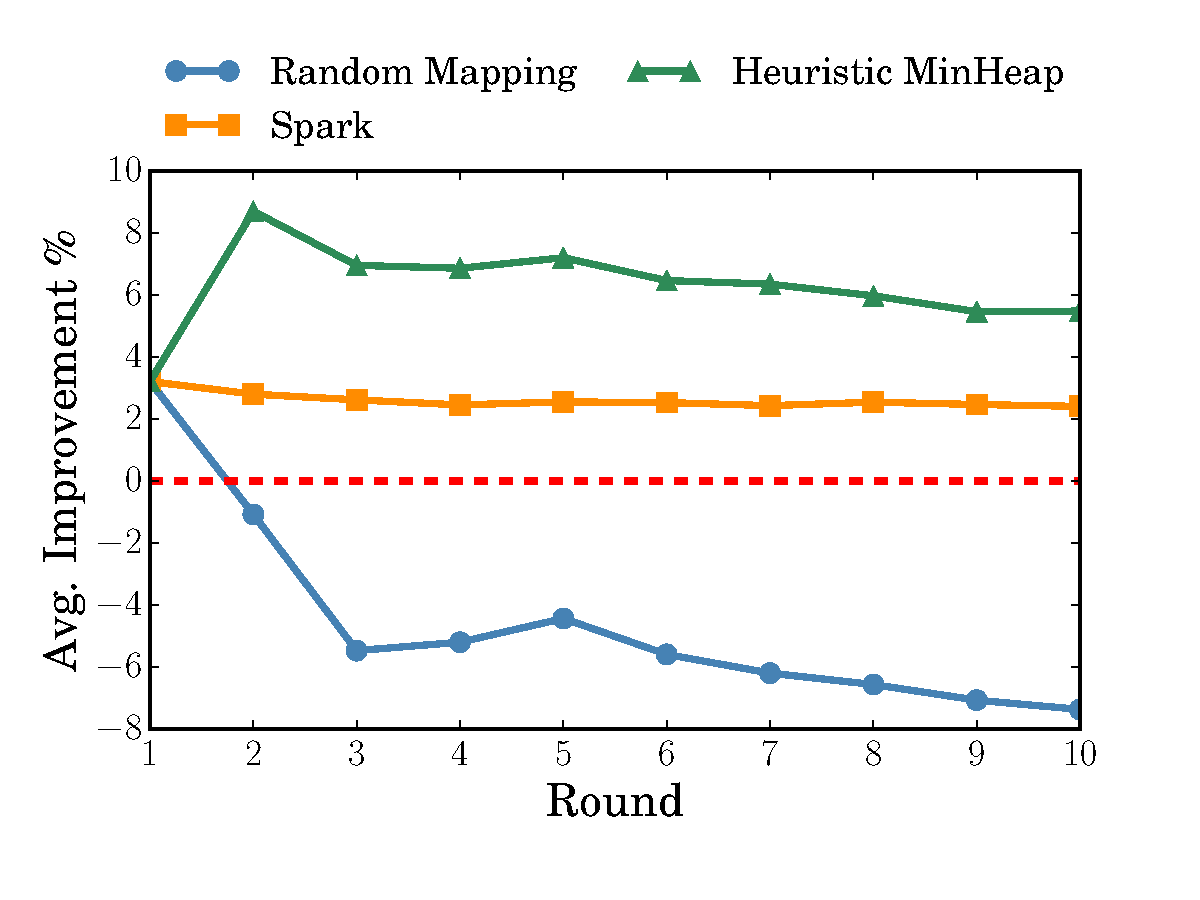
\includegraphics[width=\linewidth]{fig/sim}
% 				\caption{Stage Completion Time Improvement}
% 				\label{fig:sim}
% 			\end{subfigure}	
% 			\caption{Emulate Result of OpenCloud Trace}
% 		\end{figure}
% 	\end{minipage}
% \end{figure*}
% \begin{figure}
\subsubsection{Problem of Random Mapping}\label{randomassign}
The simplest way of pre-scheduling is mapping tasks to nodes randomly and evenly. 
In order to evaluate the effectiveness of random mapping, we use traces from OpenCloud\footnote{\label{fn:trace}http://ftp.pdl.cmu.edu/pub/datasets/hla/dataset.html} for the simulation.
% Note that most of the traces from OpenCloud are shuffle-light workload as shown in Figure \ref{fig:cdf}. 
The average shuffle read time is $3.2\%$ of total reduce completion time.


As shown in Figure \ref{fig:sim}, the baseline (i.e., red dotted line) is the stage completion time with Spark FIFO scheduling algorithm. 
We then remove the shuffle read time of each task and run the simulation under three scheduling schemes: random mapping, Spark FIFO, and our heuristic MinHeap.
Random mapping works well when there is only one round of tasks, but the performance drops as the round number grows. 
This is because that data skew commonly exists in data-parallel computing \cite{skewtune, reining, gufler2012load}. 
Several heavy tasks may be assigned to the same node, thus slowing down the whole stage. 
In addition, randomly assigned tasks also ignore the data locality between shuffle map output and reduce input, which may introduce extra network traffic in cluster.

\subsubsection{Shuffle Output Prediction}\label{shuffleprediction}
% \ifrevision
% \marginpar{B2,E7}
% \fi
The problem of random mapping is obviously caused by application context (e.g., shuffle data size) ignorance. 
Note that a balanced schedule decision can be made under the consideration of the size of each reduce task, and the size of a reduce task produced by one shuffle $reduceSize_i = \sum_{j=0}^{m} {BlockSize_{ji}}$, 
where the $m$ is the number of map tasks that can be easily extracted from DAG information; 
$BlockSize_{ji}$ represents the size of block which is produced by map $task_j$ for reduce $task_i$ (e.g., block `1-1' in Figure \ref{fig:shuffle}). 
The final sizes of reduce tasks can be calculated by aggregating $reduceSize_i$ by reduce ID among all shuffle dependencies. 
So the pre-scheduling can be made if the "prediction" of size of shuffle block is practical.
% \hlyellow{
% The shuffle size of each reduce task is decided by input data, map task computation, and hash partitioner. 
% Each map task produces a data block for each reduce task. 
% }
% The size of each reduce partition can be calculated $reduceSize_i = \sum_{j=0}^{m} {BlockSize_{ji}}$ ($m$ is the number of map tasks). 
% $BlockSize_{ji}$ represents the size of block which is produced by map $task_j$ for reduce $task_i$ (e.g., block `1-1' in Figure \ref{fig:shuffle}).
% \ifrevision
% \reversemarginpar
% \marginpar{B2,D6,D8}
% \fi

For the most DAG applications with random large scale input, 
the $BlockSize_{ji}$ in a particular shuffle can be predicted accurately by liner regression model (i.e., equation \ref{linearregresion}) based on observation that the ratio of map output size and input size are invariant given the same job configuration \cite{guo2017ishuffle, predict}: 
\begin{equation}
\label{linearregresion}
\begin{aligned}
	BlockSize_{ji} = a \times inputSize_j + b
\end{aligned}
\end{equation}
The $inputSize_j$ is the input size of $j$th map task. 
The $a$ and $b$ can be determined using the observed $inputSize_j$ and $BlockSize_{ji}$.

\begin{figure*}
	\centering
	\begin{subfigure}[b]{0.31\linewidth}
		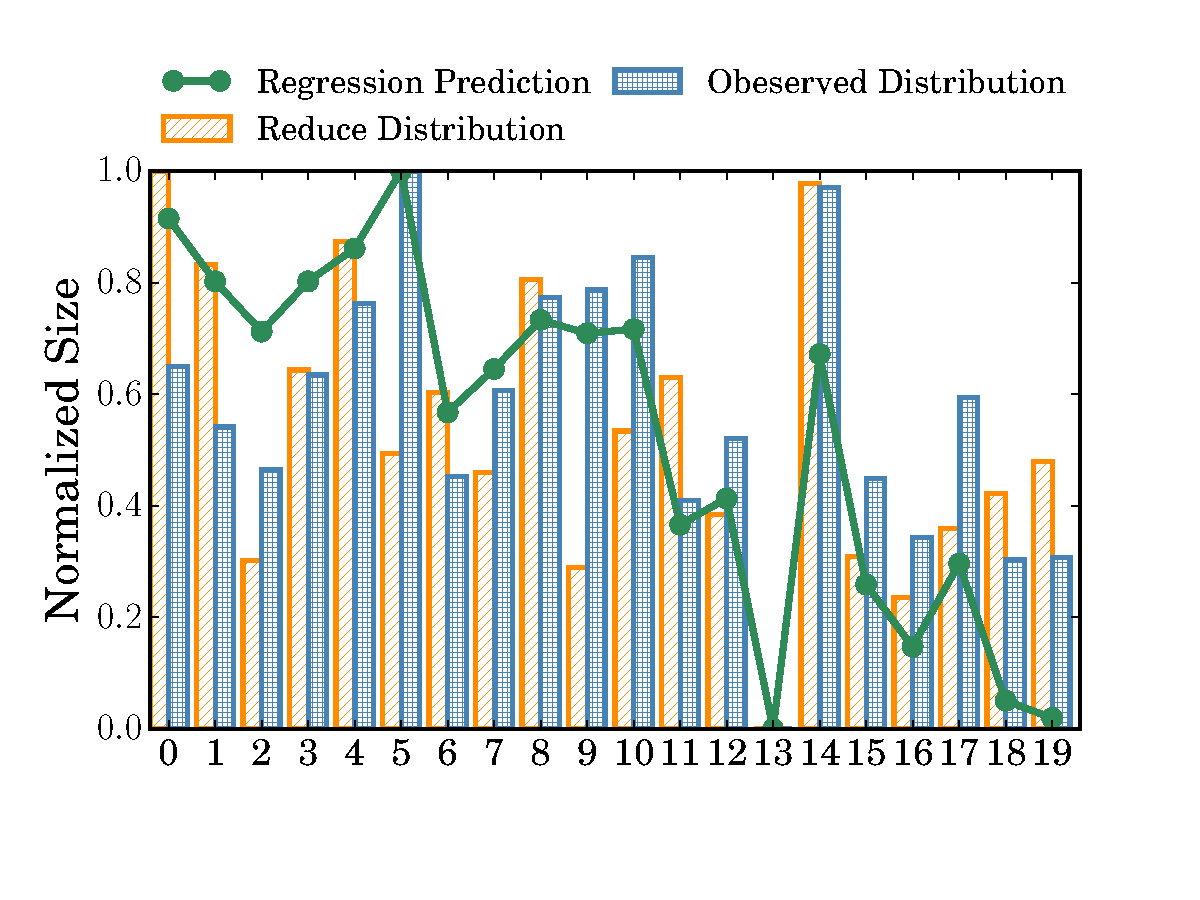
\includegraphics[width=\linewidth]{fig/hash_pre}
		\caption{Linear Regression Prediction of Hash Partitioner\newline}
		\label{fig:hash_pre}
	\end{subfigure}
	\begin{subfigure}[b]{0.31\linewidth}
		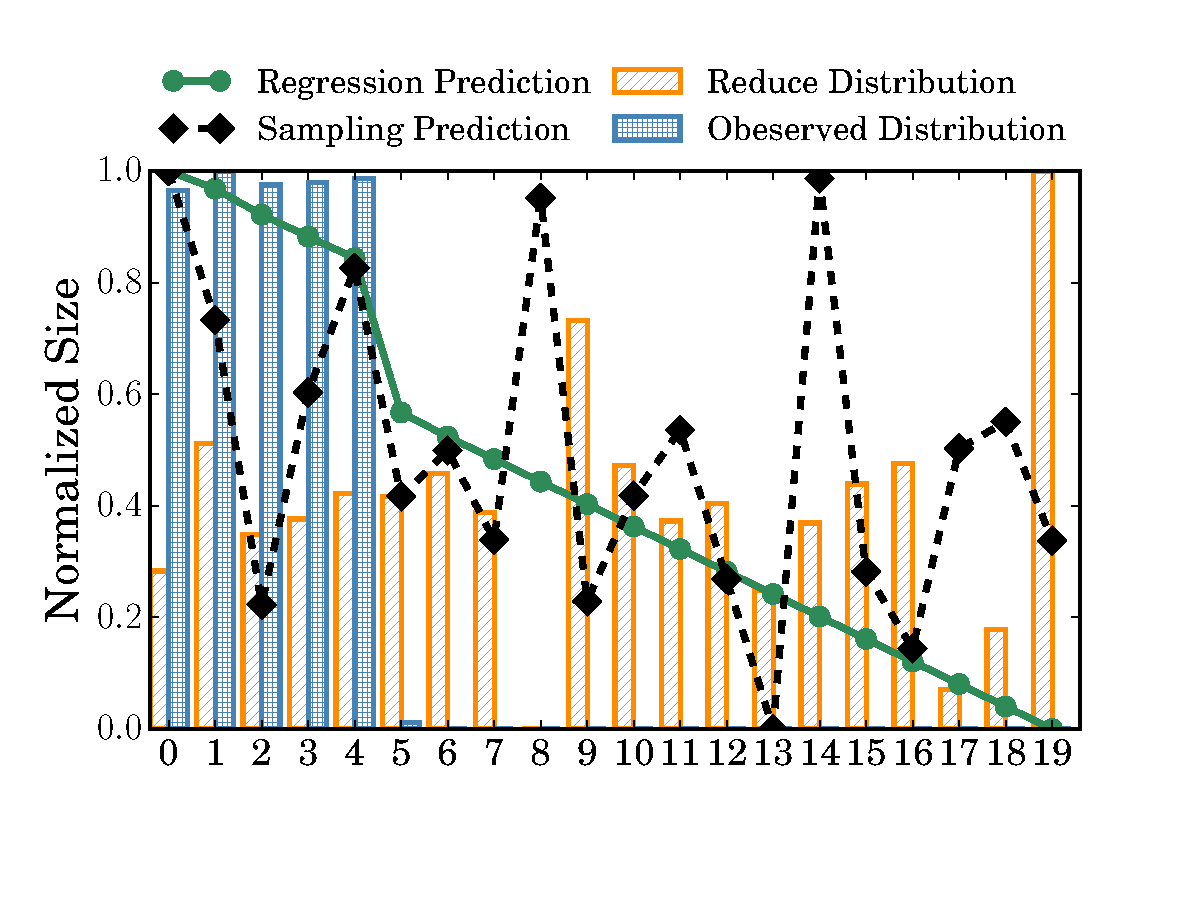
\includegraphics[width=\linewidth]{fig/range_pre_sample}
		\caption{Linear Regression and Sampling Prediction of Range Partitioner2222}
		\label{fig:range_pre_sample}
		\vspace{1em}
	\end{subfigure}
	\begin{subfigure}[b]{0.31\linewidth}
		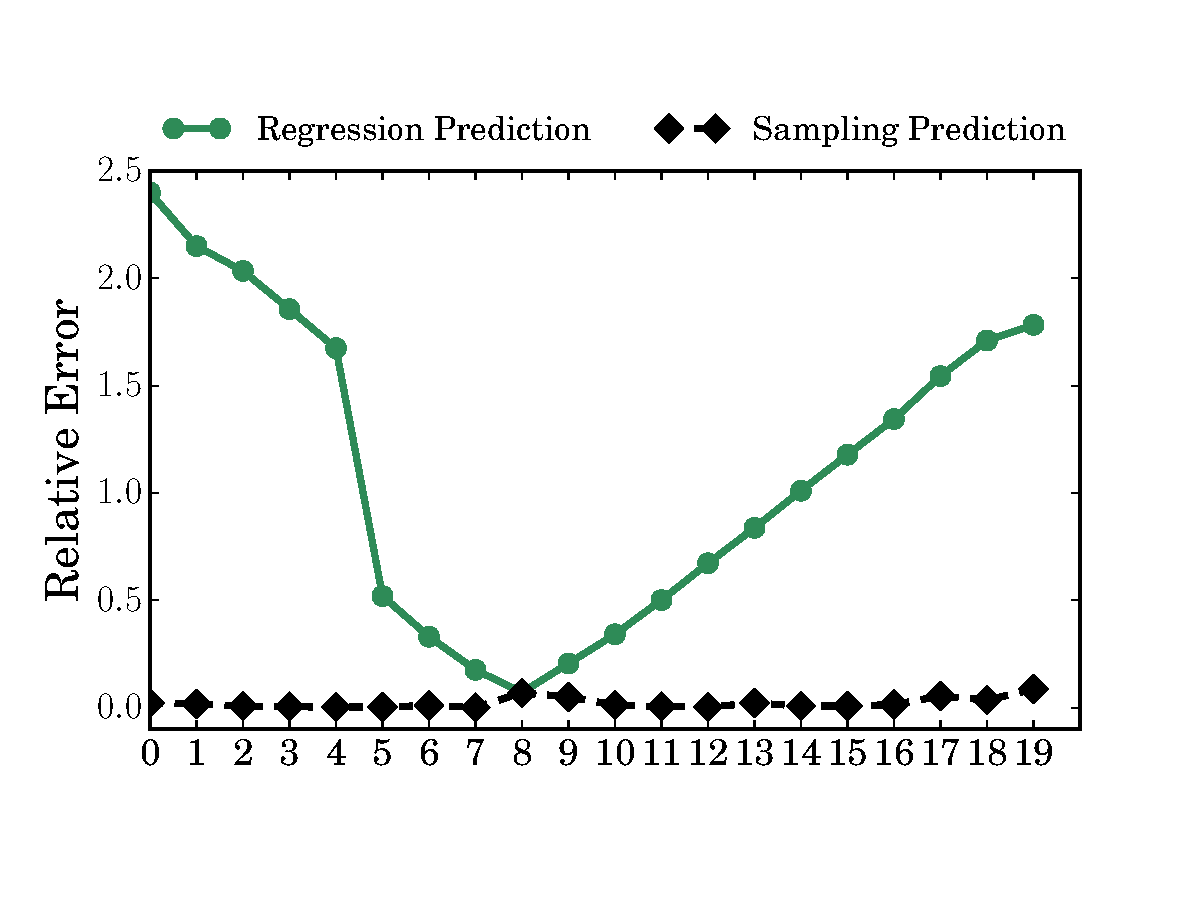
\includegraphics[width=\linewidth]{fig/prediction_relative_error}
		\caption{Prediction Relative Error of Range Partitioner\newline}
		\label{fig:prediction_relative_error}
	\end{subfigure}
	\caption{Reduction Distribution Prediction}
	\label{fig:dis}
	\vspace{-1em}
\end{figure*}

Though the linear regression is stable in most scenarios, it can fail in some uncertainties introduced by sophisticated frameworks like Spark \cite{apachespark}.  
For instance, the customized partitioner may result in large inconsistency between observed map output blocks distribution and the final reduce input distribution. 
We present two particular examples with 20 tasks respectively in Figure \ref{fig:hash_pre} and Figure \ref{fig:range_pre_sample}. 
The data in are normalized to $0-1$ because the prediction of SCache only produces the data distribution instead of the real size. 
% In Figure \ref{fig:range_pre_sample}, we use the distribution of second shuffle of Spark Terasort \cite{spark-tera} that are partitioned by Spark RangePartitioner \cite{apachespark}. 
% In Figure \ref{fig:hash_pre} and Figure \ref{fig:range_pre_sample}, we use different datasets with different partitioners, and normalize the distribution to $0-1$ to fit in one figure. 
The observed map outputs are randomly picked. 
With a random input and a hash partitioner in Figure \ref{fig:hash_pre}, the distribution of observed map output is close to the final reduce input distribution. 
The prediction results also fit them well. 
However, the data partitioned by Spark RangePartitioner \cite{apachespark} in Figure \ref{fig:range_pre_sample} results in a deviation from the linear regression model, because the RangePartitioner might introduce an extreme high data locality skew. 
That is, for one reduce task, almost all of the input data are produced by a particular map task (e.g., the observed map tasks only produce data for reduce task 0-5 in Figure \ref{fig:range_pre_sample}).
The data locality skew results in a missing of other reduce tasks' data in the observed map outputs.

% Several map outputs (marked as Map Output in Figure \ref{fig:shuffle}) are picked as observation objects to train the model and than predict the final reduce distribution.
% \ifrevision
% \reversemarginpar
% \marginpar{D6,E3}
% \fi

\noindent
\begin{minipage}{0.95\columnwidth}
\begin{algorithm}[H]
\caption{Heuristic MinHeap Scheduling for Single Shuffle}
\label{hminheap}
	\begin{algorithmic}[1]
	\small
	\Procedure{schedule}{$m, host\_ids, p\_reduces$}
		\State $m\gets$ partition number of map tasks
		\State $R\gets$ sort $p\_reduces$ by size in non-increasing order
		\State $M\gets$ min-heap $\left\{ host\_id \rightarrow \left( \left[ reduces \right], size \right) \right\}$
		\State $idx\gets 0$
		\While{$idx <$ len$R$}
		% \Comment{Schedule reduces by MinHeap}
		\State $M\left[0\right].size \mathrel{+}= R\left[idx\right].size$
		\State $M\left[0\right].reduces.append\left(R\left[idx\right]\right)$
		\State $R\left[idx\right].assigned\_id \gets M \left[0\right].host\_id$
		\State Sift down $M\left[0\right]$ by $size$
		\State $idx\gets idx-1$
		\EndWhile
		\State $max\gets$ maximum size in $M$
		% \State Convert $M$ to mapping $\left\{ host\_id \rightarrow \left( \left[ rid\_arr \right], size \right) \right\}$
		\ForAll{$reduce$ in $R$}
		\Comment{Heuristic locality swap}
			\If{$reduce.assigned\_id \neq reduce.host\_id$}
				\State $p\gets reduce.prob$
				\State $norm\gets \left(p-1/m\right)/\left(1-1/m\right)/10$
				\State $upper\_bound \gets \left(1 + norm\right) \times max$
				\State SWAP\_TASKS$\left(M, reduce, upper\_bound\right)$
			\EndIf
		\EndFor
		\Return $M$
	\EndProcedure
	\Procedure{swap\_tasks}{$M, reduce, upper\_bound$}
		\State Swap tasks between node $host\_id$ and node $assigned\_id$
		\State of $reduce$ without exceeding the $upper\_bound$
		\State of both nodes.
		\State Return if it is impossible.
	\EndProcedure
	\end{algorithmic}
\end{algorithm}
\end{minipage}

To handle this corner case, we introduce another methodology, named \emph{weighted reservoir sampling}, as a substitution of linear regression. 
Note that linear regression will be replaced only when a RangePartitioner or a customized non-hash partitioner occurs. 
For each map task, we use classic reservoir sampling to randomly pick $s \times p$ of samples, where $p$ is the number of reduce tasks and $s$ is a tunable number. 
After that, the map function is called locally to process the sampled data (\textit{Sampling} in Figure \ref{fig:shuffle}). 
Finally, the partitioned outputs are collected with the $InputSize_j$ as the weight of the samples.
Note that sampling does not consume the input data of map tasks. 
The $BlockSize_{ji}$ can be calculated by:
\begin{equation}
\label{equationsample}
\begin{aligned}
	BlockSize_{ji} &= {{InputSize_j \times \frac{sample_i}{s \times p}}} \\
	sample_i &= \text{number of samples for $reduce_i$}
\end{aligned}
\end{equation}
% The classic reservoir sampling is designed for randomly choosing \textit{k} samples from \textit{n} items, where \textit{n} is either a very large or an unknown number \cite{reservoir}. 
In Figure \ref{fig:range_pre_sample}, when $s$ is set to $3$, the result of sampling prediction is much better than linear regression. 
The variance of the normalization between sampling prediction and reduce distribution is because the standard deviation of the prediction results is relatively small compared to the average prediction size, which is $0.0015$ in this example. 
Figure \ref{fig:prediction_relative_error} further proves that the sampling prediction can provide precise result even in the dimension of absolute input size of reduce task. 
On the other hand, the result of linear regression comes out with a large relative error. 
Though the weighted reservoir sampling is precise, it also introduced extra overhead. 
We will show the overhead evaluation of sampling in Section \ref{evaluation}.
% {\color{blue}
% Figure \ref{fig:prediction_relative_error} proves that the sampling prediction can provide much more accurate result than the linear regression. 
% We will show the overhead evaluation of sampling in Section \ref{evaluation}. 
% }

During both of the predictions, the composition of each reduce partition is calculated as well. We define $prob_i$ as
\begin{equation}
\label{equationprob}
\begin{aligned}
	prob_i &= \max_{0 \leq j \leq m} \frac{BlockSize_{kji}}{reduceSize_i} \\
    m &= \text{number of map tasks}
\end{aligned}
\end{equation}
This parameter is used to achieve a better data locality while performing shuffle pre-scheduling. 


\subsubsection{Heuristic MinHeap Scheduling}\label{h-minheap}

% \ifrevision
% \marginpar{\tiny PC2,C1,D7/9,E4}
% \fi
As long as the input sizes of reduce tasks are available, the pre-scheduling is a classic scheduling problem without considering the data locality. 
But ignoring the data locality can introduce extra network transfer. 
In order to balance load while minimizing the network traffic, we present the Heuristic MinHeap scheduling algorithm (Algorithm \ref{hminheap}).   

For the pre-scheduling itself (i.e., the first $while$ in Algorithm \ref{hminheap}), the algorithm maintains a min-heap to simulate the load of each node 
and applies the longest processing time rule (LPT) \cite{design} to achieve $4/3\text{-}approximation$ optimum. 
Since the sizes of tasks are considered while scheduling, Heuristic MinHeap can achieve a shorter makespan than Spark FIFO which is a $2\text{-}approximation$ optimum. 
Simulation of OpenCloud trace in Figure \ref{fig:sim} also shows that Heuristic MinHeap has a better improvement (average 5.7\%) than the Spark FIFO (average 2.7\%).
% After the scheduling, the completion time of reduce stage is close to the optimal. \textcolor{red}{may need to add math prove between this and optimal}.
After pre-scheduling, the task-node mapping will be adjusted according to the locality. 
The $SWAP\_TASKS$ will be triggered when the $host\_id$ of a task does not equal the $assigned\_id$.
% The closer $prob$ is to $1/m$, the more evenly this reduce partition is produced in cluster.
Based on the $prob$, the normalized probability $norm$ is calculated as a bound of performance degradation. 
% We set maximum $upper\_bound$ of performance degradation equals to 10\% that can be traded for locality (in extreme skew scenarios).
Inside the $SWAP\_TASKS$, tasks will be selected and swapped without exceeding the $upper\_bound$. 

\subsubsection{Cope with Multiple Shuffle Dependencies}
% \ifrevision
% \marginpar{E5}
% \fi
A reduce stage can have more than one shuffle dependencies in the current DAG computing frameworks. 
The technique mentioned in Section \ref{shuffleprediction} can only handle an ongoing shuffle. 
For those pending shuffles, it is impossible to predict their sizes. 
This problem can be solved by having all map tasks of pending shuffles launched simultaneously. 
But doing this introduces large overhead such as extra task serialization. 
To avoid violating the optimization from framework, we present the Accumulated Heuristic Scheduling algorithm to cope with multiple shuffle dependencies.

As illustrated in Algorithm \ref{mhminheap}, the sizes of previous \emph{shuffles} scheduled by Heuristic MinHeap are counted. 
When a new shuffle starts, the predicted $size$, $prob$, and $host\_id$ in $p\_reduces$ are accumulated with previous \emph{shuffles}. 
After scheduling, if the new $assigned\_id$ of a reduce task did not equal the original one, a re-shuffle will be triggered to transfer data to the new host. 
This re-shuffle is rare since the previous shuffle data contributes a huge composition (i.e., high $prob$) after the accumulation, 
which leads to a higher probability of tasks swap in $SWAP\_TASKS$. 

\noindent
\begin{minipage}{0.95\columnwidth}
\begin{algorithm}[H]
\caption{Accumulated Heuristic Scheduling for Multi-Shuffles}
\label{mhminheap}
	\begin{algorithmic}[1]
	\small
	\Procedure{m\_schedule}{$m, host\_id, p\_reduces, \text{\emph{shuffles}}$}
		\State $m\gets$ partition number of map tasks
		\Comment \emph{shuffles} are the previous schedule result 
		\ForAll{$r$ in $p\_reduces$}
			\State $r.size \mathrel{+}= \text{\emph{shuffles}}\left[r.rid\right].size$
			\State $new\_prob\gets \text{\emph{shuffles}}\left[r.rid\right].size / r.size$
			\If{$new\_prob\geq r.prob$}
				\State $r.prob\gets new\_prob$
				\State $r.host\_id\gets \text{\emph{shuffles}}\left[r.rid\right].assigned\_host$
			\EndIf
		\EndFor
		\State $M\gets$ $SCHEDULE\left(m, host\_id, p\_reduces\right)$
		\ForAll{$host\_id$ in $M$}
			\Comment Re-shuffle
			\ForAll{$r$ in $M\left[host\_id\right].reduces$}
				\If{$host\neq \text{\emph{shuffles}}\left[r.rid\right].assigned\_host$}
				\State Re-shuffle data to $host$
				\State $\text{\emph{shuffles}}\left[r.rid\right].assigned\_host\gets host$
				\EndIf
			\EndFor
		\EndFor
		\Return $M$
	\EndProcedure
	\end{algorithmic}
\end{algorithm}
\end{minipage}

% It means the $SWAP\_TASKS$ can help revise the scheduling to match the previous mapping as much as possible while maintaining the good load balance.

% As for the input of $SCHEDULE$ function in Algorithm \ref{hminheap}, $m$ is the partition number of input data; $h$ is the array of nodes ID in cluster; $p\_reduces$ is the predicted reduce matrix. Each row in $p\_reduces$ contains $rid$ as reduce partition ID; $size$ as predicted size of this partition; $prob$ as the maximum composition portion of reduce data; $host\_id$ as the node ID that produces the maximum portion of reduce data, and $assigned\_id$ as the node ID assigned by Algorithm \ref{hminheap}. As for $M$, it is consists $host\_id$, an array of $reduce$ scheduled on this node and the $size$ of them.
